\documentclass[a4paper,12pt]{article}
% \input{../../../config.tex}
\usepackage{../../mypackages}
\usepackage{../../macros}


\usepackage{pgfplots}
    \pgfplotsset{
    compat=1.11,
  }

\usetikzlibrary{shapes,arrows,babel}
\tikzstyle{box}=[minimum size = 0.1cm, rectangle, draw=black, fill=gray]
% Define the global variable

% Function that meets the requirements + ways to do custom drawing
% https://tex.stackexchange.com/questions/490374/a-curve-pass-via-points-at-tikz


\def\WITH_CORRECTION{YES}


\begin{document}

\title{Physique-Chimie - Rappels de 2nde}
\author{N. Bancel}

\sloppy  % This will apply the sloppy setting to the entire document.
\maketitle

\section{Corps purs et mélanges}

\begin{enumerate}
  \item Définition d'un corps pur ? D'un mélange ?
  \ans{
    Un corps pur est une substance constituée d'une seule espèce chimique (atomes, molécules, ou ions), par exemple l'eau pure (H\textsubscript{2}O). \par
    Un mélange est une substance constituée de plusieurs espèces chimiques. Par exemple, l'air est un mélange de diazote (N\textsubscript{2}), de dioxygène (O\textsubscript{2}) et d'autres gaz.
  }{1}{FALSE}
  \item Comment s'exprime le pourcentage massique ? Le pourcentage volumique ? Quelle est la proportion volumique du diazote dans l'air ? Et du dioxygène ? \par
  \ans{
    Le pourcentage massique s'exprime par la relation suivante : \[ \text{Pourcentage massique} = \frac{\text{masse du constituant}}{\text{masse totale du mélange}} \]
    Le pourcentage volumique s'exprime par la relation suivante : \[ \text{Pourcentage volumique} = \frac{\text{volume du constituant}}{\text{volume total du mélange}} \]
    La proportion volumique du diazote (N\textsubscript{2}) dans l'air est d'environ 78\%. Celle du dioxygène (O\textsubscript{2}) est d'environ 21\%.
  }{1}{FALSE}
  \item Quelle est l'expression de la masse volumique ? \par
  \ans{La masse volumique (ou densité de masse) est définie comme la masse par unité de volume. Elle s'exprime par la formule : 
  \[
  \rho = \frac{m}{V}
  \]
  où $\rho$ est la masse volumique en kg/m$^3$, $m$ est la masse en kg, et $V$ est le volume en m$^3$.}{1}{FALSE}
\end{enumerate}


\section{Solutions aqueuses}
\begin{enumerate}
  \item Quelle est la définition d'une solution ? D'une solution aqueuse ?
  \ans{Une solution est un mélange homogène composé d'un soluté dissous dans un solvant.
  La solvant est l'espèce chimique majoritaire. \par
  Le soluté est l'espère chimique minoritaire. \par
  Une solution aqueuse est une solution où le solvant est l'eau.}{1}{FALSE}
  \item Quelle est la définition de la concentration en masse ? Des exemples quotidiens dans lesquels on quantifie la concentration en masse ?
  \ans{La concentration en masse est la quantité de soluté (en grammes) dissoute dans un certain volume de solution (en litres). Elle s'exprime par la formule : 
  \[
  C_m = \frac{m_\text{soluté}}{V_\text{solution}}
  \]
  Des exemples quotidiens incluent la concentration de sucre dans une boisson ou la quantité de sel dans l'eau de mer.}{1}{FALSE}
  \item Quelle est la différence entre la masse volumique, et la concentration en masse ?
  \ans{Bien que leur unité soit la même : la masse volumique mesure la quantité de masse d'un matériau par unité de volume ($\rho = \frac{m}{V}$), tandis que la concentration en masse se réfère à la quantité de soluté dissous dans un volume de solution ($C_m = \frac{m_\text{soluté}}{V_\text{solution}}$). La première concerne les substances pures, la seconde s'applique aux solutions.}{1}{FALSE}
\end{enumerate}



\section{De l'atome à l'élément chimique}

\begin{enumerate}
  \item De quoi est constituté un atome ? Que peut-on dire de sa charge électrique ?
  \ans{
    \begin{itemize}
      \item[$\bullet$] Un atome est constitué d'un noyau chargé positivement et d'électrons chargés négativement en mouvement désordonné autour de ce noyau.
      \item[$\bullet$] Un atome est donc électriquement neutre car il possède autant de protons que d'électrons.
    \end{itemize} \par 
    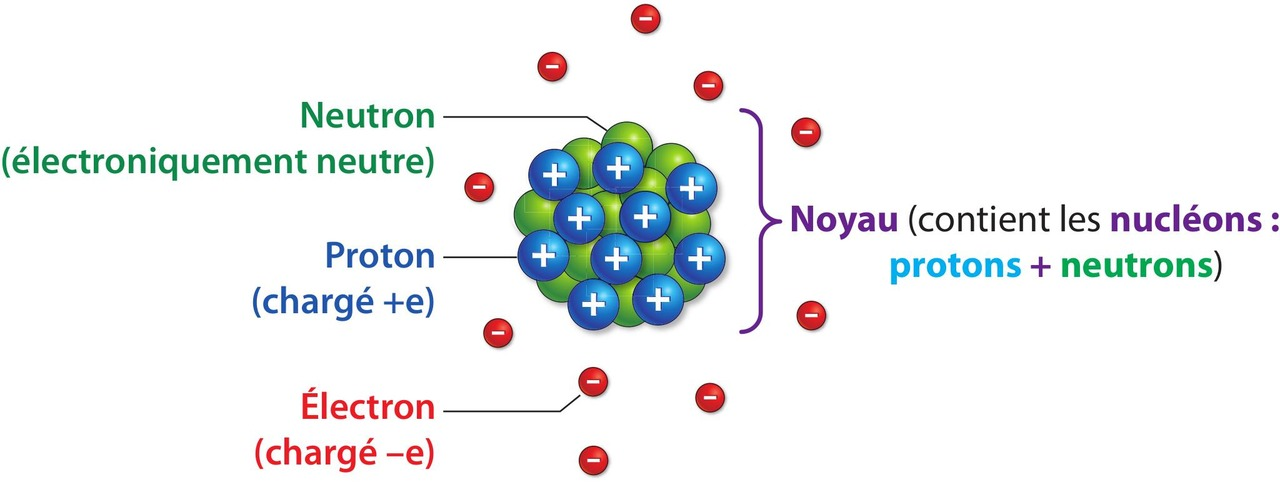
\includegraphics[width=\textwidth]{atome.jpg}
    \captionof{figure}{Structure de l'atome}
    }{1}{FALSE}
  \item Quelle est l'écriture conventionnelle du noyau d'un atome de symbole X ? \par
  \ans{ 
    \begin{figure}[H]
      \centering
      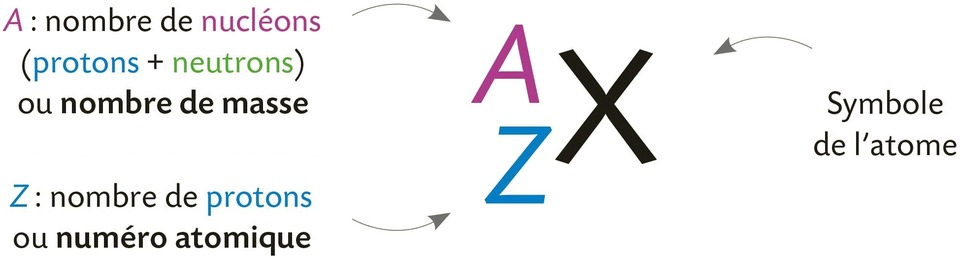
\includegraphics[width=0.5\linewidth]{symbole_atome.jpg}
      \caption{\label{fig:symbole_atome} Structure de l'atome}
  \end{figure} \par 
    \vspace{1em} % Ajoute un espace vertical de 1em
    (Le nombre de neutrons est donc égal à \(A – Z\)).
    }{1}{FALSE}
    \item Qu'est ce qu'un ion monoatomique ? \par
    \ans{
      \begin{tcolorbox}
        Un ion monoatomique se forme lorsqu'un atome gagne ou perd un ou plusieurs électrons.
      \end{tcolorbox}
      \begin{center}
        \begin{tabularx}{\textwidth}{||X X||}
          \hline
          Anion & Cation \\
          \hline
          \ce{Cl-} : Ion de charge négative & \ce{Mg^2+} : Ion de charge positive \\
          \hline
          Formé à partir d'un atome de chlore \ce{Cl} qui gagne un électron & Formé à partir d'un atome de magnésium \ce{Mg} qui perd 2 électrons \\
          \hline
        \end{tabularx}
        \end{center}
    }{1}{FALSE}
  \end{enumerate}

    \section{Vers des entités plus stables}
  \begin{enumerate}
    \item\ Comment les électrons se répartissent-ils autour de l'atome ?
    \ans{
      Les électrons se répartissent autour du noyau atomique selon des couches électroniques et des sous-couches. Voici une description détaillée de cette organisation. \par 
      Les électrons occupent des \textbf{couches électroniques}, notées  de \(n = 1, 2, 3\) etc
      Chaque couche électronique est divisée en \textbf{sous-couches} qui sont notées par les lettres \(s\), \(p\), etc.
      \begin{itemize}
        \item La sous-couche \(s\) peut contenir jusqu'à 2 électrons.
        \item La sous-couche \(p\) peut contenir jusqu'à 6 électrons.
    \end{itemize}
    \begin{figure}[H]
      \centering
      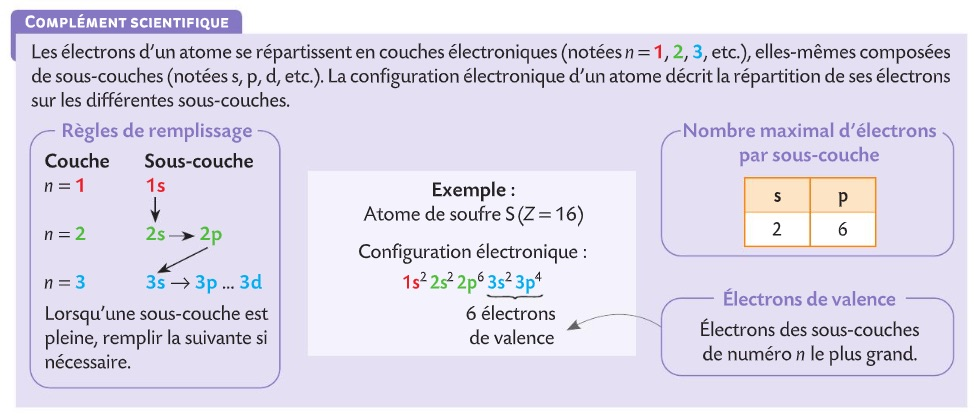
\includegraphics[width=0.5\linewidth]{config_electronique.jpg}
      \caption{\label{fig:config_electronique} Configuration électronique de l'atome}
  \end{figure}
    }{1}{FALSE}

    \item\ Quelle est la configuration électronique de l'atome de magnésium \ce{Mg} (numéro atomique = 12) ? Combien a-t-il d'électrons de valence ? \par
    \ans{
      \[
      \textcolor{red}{1s^2} \, \textcolor{green}{2s^2 \, 2p^6} \, \textcolor{blue}{3s^2}
      \] \par 
      Il y a donc 2 électrons de valence. 
    }{1}{FALSE}

    \item\ Quelle est la configuration électronique de l'atome de magnésium \ce{Cl} (numéro atomique = 17) ? Combien a-t-il d'électrons de valence ? \par
    \ans{
      \[
      \textcolor{red}{1s^2} \, \textcolor{green}{2s^2 \, 2p^6} \, \textcolor{blue}{3s^2 \, 3p^5}
      \] \par 
      Il y a donc 7 électrons de valence. 
    }{1}{FALSE}
    \item\ Qu'est ce que le tableau périodique des éléments ?
    \ans{
      Le \textbf{tableau périodique des éléments}, aussi appelé \textbf{tableau de Mendeleïev}, est un tableau qui regroupe tous les éléments chimiques connus, comme l'oxygène, le fer ou encore l'hydrogène. Il est organisé de manière à montrer les propriétés des éléments et leurs relations entre eux. \par      
      Les éléments chimiques sont classés dans le tableau périodique en fonction de leur \textbf{numéro atomique}, c'est-à-dire le nombre de protons dans leur noyau. Les éléments sont disposés en \textbf{lignes} et en \textbf{colonnes} selon leurs propriétés chimiques.
      \begin{itemize}
          \item Les \textbf{lignes horizontales} sont appelées des \textbf{périodes}. Chaque période correspond à une couche électronique.
          \item Les \textbf{colonnes verticales} sont appelées des \textbf{familles} ou \textbf{groupes}. Les éléments d'une même colonne ont des propriétés similaires, car ils ont le même nombre d'électrons sur leur dernière couche (appelée \textbf{couche de valence}).
      \end{itemize}
      \begin{figure}[H]
        \centering
        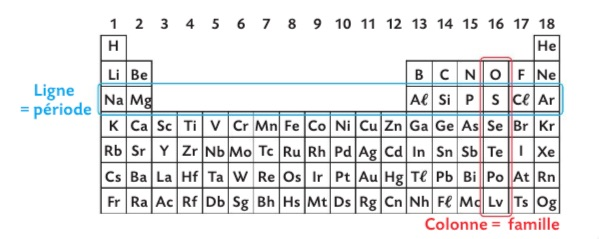
\includegraphics[width=0.5\linewidth]{periodique.jpg}
        \caption{\label{fig:periodique} Tableau périodique des éléments}
      \end{figure}
    }{1}{FALSE}
 \end{enumerate}

    \section{Quantité de matière}
    \begin{enumerate}
      \item Comment calcule-t-on la masse d'une entité ? (atome, ion, molécule) \par 
    \ans{
      La masse \(m_{entité}\) d'une entité est égale à la masse des atomes qui la composent.
      \textbf{Formule brute} du dioxyde de carbone : \ce{CO2} (1 atome de carbone, 2 atomes d'oxygène)

      \[
     m(\text{CO}_2) = m_{\text{C}} + 2 \times m_{\text{O}}
      \]
    }{1}{FALSE}
      \item Comment détermine-t-on le nombre d'entités présentes dans un échantillon dont on connaît la masse ? Par exemple, comment faire pour connaître le nombre d'atomes de carbones contenu dans une mine de crayon en carbon de 2 grammes ?
      \ans{
          \[
      N = \frac{m}{m_{\text{entité}}}
      \]
      \begin{itemize}
        \item \(N\) est le nombre d'entités dans l'échantillon
        \item \(m\) est la masse de l'échantillon en kg
        \item  \(m_{\text{entité}}\) est la masse de l'entité en kg
      \end{itemize}
      }{1}{FALSE}

      \item Avec des mots simples, expliquer le concept de quantité de matière, et son intérêt. \par
      \ans{
        Le nombre d'entité (N) est beaucoup trop élevé pour être palpable. On essaie donc de se ramener à des ordres de grandeur plus compréhensibles.
        C'est le même principe que pour les années lumières ou les unités astronomiques en astro physique.
        On regroupe donc les entités en "paquets" appelés "moles" 

        1 mole contient \(6.02 * 10^{23}\) entités.

        La constante d'Avogadro est donnée par :

        \[N_A = \SI{6.02e23}{\per\mol}\]

      }{1}{FALSE}
  \end{enumerate}

  \end{document}
